%!TEX TS-program = xelatex
\documentclass[12pt, a4paper]{article}  
\usepackage{etex} % расширение классического tex в частности позволяет подгружать гораздо больше пакетов, чем мы и займёмся далее

%%%%%%%%%% Математика %%%%%%%%%%
\usepackage{amsmath,amsfonts,amssymb,amsthm,mathtools} 

%%%%%%%%%%%%%%%%%%%%%%%% Шрифты %%%%%%%%%%%%%%%%%%%%%%%%%%%%%%%%%
\usepackage{fontspec}         % пакет для подгрузки шрифтов
\setmainfont{Arial}   % задаёт основной шрифт документа
\defaultfontfeatures{Mapping=tex-text}
\newfontfamily{\cyrillicfonttt}{Arial}
\newfontfamily{\cyrillicfont}{Arial}
\newfontfamily{\cyrillicfontsf}{Arial}
\usepackage{unicode-math}     % пакет для установки математического шрифта
\setmathfont{Asana Math}      % шрифт для математики

\usepackage{polyglossia}      % Пакет, который позволяет подгружать русские буквы
\setdefaultlanguage{russian}  % Основной язык документа
\setotherlanguage{english}    % Второстепенный язык документа

%%%%%%%%%% Работа с картинками %%%%%%%%%
\usepackage{graphicx}                  % Для вставки рисунков
\usepackage{graphics}
\graphicspath{{images/}{pictures/}}    % можно указать папки с картинками
\usepackage{wrapfig}                   % Обтекание рисунков и таблиц текстом
\usepackage{subfigure}                 % для создания нескольких рисунков внутри одного

%%%%%%%%%% Графика и рисование %%%%%%%%%%
\usepackage{tikz, pgfplots}  % язык для рисования графики из latex'a
\usepackage{amscd}                  %Пакеты для рисования
\usepackage[matrix,arrow,curve]{xy} %комунитативных диаграмм

% Всякие команды из Geogebra
\usepackage{pgf}
\usepackage{mathrsfs}
\usetikzlibrary{arrows}
\pagestyle{empty}
\definecolor{qqqqff}{rgb}{0.,0.,1.}
\definecolor{zzttqq}{rgb}{0.6,0.2,0.}

\author{Кунакбаева Камила}
\title{Упражнение 2}
\date{\today}

\begin{document}

\maketitle

\newenvironment{spherkon}{\hrule\begin{center}}%
{\end{center}\smallskip\hrule
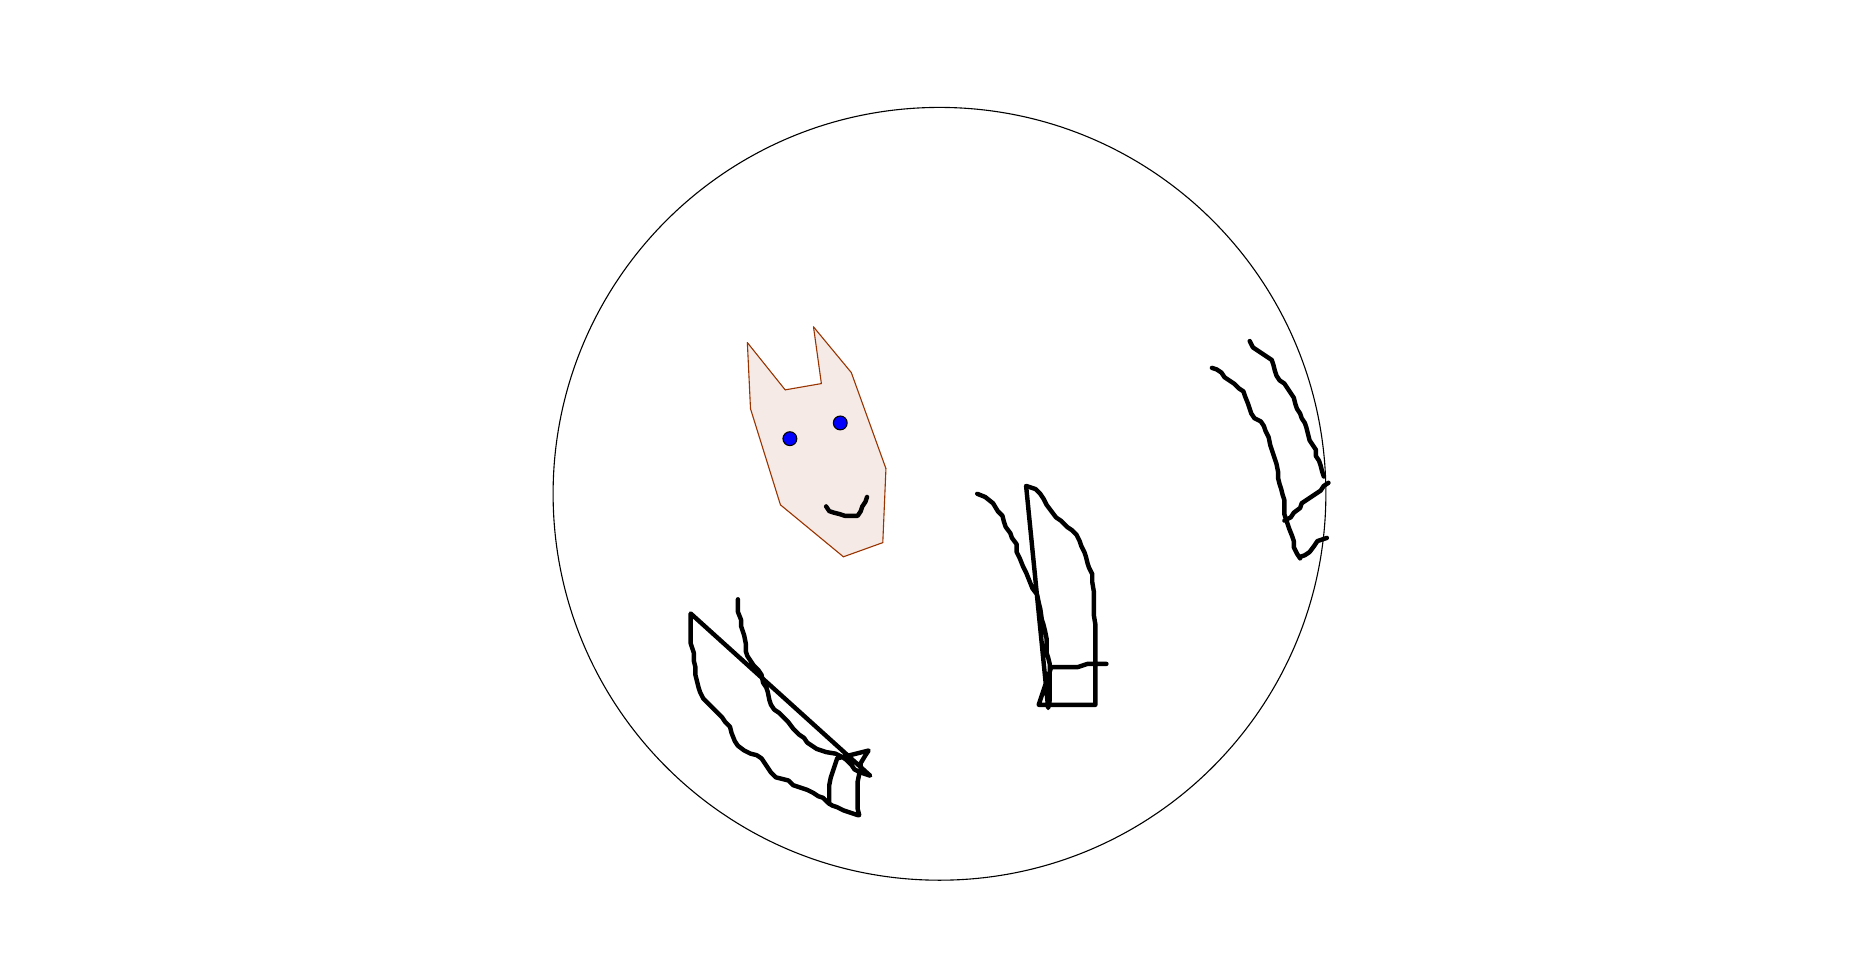
\begin{tikzpicture}[line cap=round,line join=round,>=triangle 45,x=1.0cm,y=1.0cm]
\clip(-3.36,0.08) rectangle (19.64,11.72);
\fill[color=zzttqq,fill=zzttqq,fill opacity=0.10000000149011612] (5.82,6.88) -- (6.2,5.66) -- (7.,5.) -- (7.5,5.18) -- (7.54,6.12) -- (7.1,7.34) -- (6.62,7.92) -- (6.72,7.2) -- (6.26,7.12) -- (5.78,7.72) -- cycle;
\draw(8.22,5.8) circle (4.90717841534216cm);
\draw [color=zzttqq] (5.82,6.88)-- (6.2,5.66);
\draw [color=zzttqq] (6.2,5.66)-- (7.,5.);
\draw [color=zzttqq] (7.,5.)-- (7.5,5.18);
\draw [color=zzttqq] (7.5,5.18)-- (7.54,6.12);
\draw [color=zzttqq] (7.54,6.12)-- (7.1,7.34);
\draw [color=zzttqq] (7.1,7.34)-- (6.62,7.92);
\draw [color=zzttqq] (6.62,7.92)-- (6.72,7.2);
\draw [color=zzttqq] (6.72,7.2)-- (6.26,7.12);
\draw [color=zzttqq] (6.26,7.12)-- (5.78,7.72);
\draw [color=zzttqq] (5.78,7.72)-- (5.82,6.88);
\draw [line width=1.6pt] (8.7,5.8)-- (8.7,5.8)-- (8.7,5.8)-- (8.8,5.76)-- (8.9,5.68)-- (8.96,5.58)-- (9.02,5.52)-- (9.04,5.44)-- (9.06,5.38)-- (9.12,5.3)-- (9.14,5.24)-- (9.2,5.16)-- (9.2,5.06)-- (9.24,4.98)-- (9.28,4.88)-- (9.32,4.8)-- (9.36,4.7)-- (9.4,4.6)-- (9.46,4.52)-- (9.48,4.42)-- (9.5,4.34)-- (9.52,4.2)-- (9.54,4.14)-- (9.56,4.06)-- (9.58,3.96)-- (9.58,3.88)-- (9.58,3.78)-- (9.6,3.72)-- (9.62,3.64)-- (9.62,3.56)-- (9.62,3.46)-- (9.62,3.36)-- (9.62,3.28)-- (9.62,3.18)-- (9.6,3.08)-- (9.32,5.9)-- (9.32,5.9)-- (9.32,5.9)-- (9.32,5.9)-- (9.38,5.88)-- (9.44,5.86)-- (9.5,5.8)-- (9.54,5.74)-- (9.58,5.66)-- (9.64,5.58)-- (9.7,5.5)-- (9.76,5.46)-- (9.84,5.38)-- (9.9,5.34)-- (9.96,5.28)-- (10.,5.2)-- (10.02,5.14)-- (10.06,5.06)-- (10.08,5.)-- (10.1,4.92)-- (10.12,4.86)-- (10.16,4.78)-- (10.16,4.68)-- (10.18,4.56)-- (10.18,4.44)-- (10.18,4.34)-- (10.18,4.26)-- (10.2,4.14)-- (10.2,3.98)-- (10.2,3.88)-- (10.2,3.76)-- (10.2,3.62)-- (10.2,3.5)-- (10.2,3.4)-- (10.2,3.32)-- (10.2,3.24)-- (10.2,3.16)-- (10.2,3.16)-- (10.2,3.12)-- (10.2,3.12)-- (10.2,3.12)-- (10.08,3.12)-- (10.,3.12)-- (9.9,3.12)-- (9.82,3.12)-- (9.72,3.12)-- (9.64,3.12)-- (9.56,3.12)-- (9.48,3.12)-- (9.48,3.12)-- (9.64,3.6)-- (9.64,3.6)-- (9.64,3.6)-- (9.72,3.6)-- (9.8,3.6)-- (9.88,3.6)-- (9.98,3.6)-- (10.04,3.62)-- (10.1,3.64)-- (10.18,3.64)-- (10.26,3.64)-- (10.34,3.64);
\draw [line width=1.6pt] (5.66,4.46)-- (5.66,4.46)-- (5.66,4.46)-- (5.66,4.38)-- (5.66,4.3)-- (5.7,4.2)-- (5.7,4.12)-- (5.74,4.)-- (5.76,3.9)-- (5.76,3.8)-- (5.78,3.74)-- (5.82,3.68)-- (5.86,3.62)-- (5.92,3.56)-- (5.96,3.5)-- (5.98,3.4)-- (6.02,3.34)-- (6.04,3.28)-- (6.06,3.18)-- (6.08,3.12)-- (6.12,3.06)-- (6.18,3.02)-- (6.24,2.96)-- (6.3,2.9)-- (6.36,2.82)-- (6.44,2.74)-- (6.5,2.7)-- (6.54,2.64)-- (6.6,2.6)-- (6.66,2.56)-- (6.72,2.54)-- (6.78,2.52)-- (6.9,2.5)-- (6.98,2.46)-- (7.04,2.42)-- (7.1,2.36)-- (7.14,2.3)-- (7.22,2.26)-- (7.28,2.24)-- (7.34,2.22)-- (7.34,2.22)-- (5.06,4.28)-- (5.06,4.28)-- (5.06,4.28)-- (5.06,4.2)-- (5.06,4.1)-- (5.06,4.)-- (5.06,3.9)-- (5.08,3.84)-- (5.1,3.78)-- (5.1,3.68)-- (5.12,3.6)-- (5.12,3.5)-- (5.14,3.42)-- (5.16,3.34)-- (5.18,3.28)-- (5.22,3.2)-- (5.28,3.14)-- (5.34,3.08)-- (5.4,3.02)-- (5.46,2.96)-- (5.5,2.9)-- (5.56,2.84)-- (5.58,2.76)-- (5.62,2.66)-- (5.66,2.6)-- (5.74,2.54)-- (5.82,2.5)-- (5.9,2.48)-- (5.96,2.44)-- (6.,2.38)-- (6.04,2.32)-- (6.08,2.26)-- (6.14,2.2)-- (6.22,2.18)-- (6.3,2.16)-- (6.36,2.1)-- (6.42,2.08)-- (6.48,2.06)-- (6.54,2.04)-- (6.62,2.)-- (6.68,1.96)-- (6.74,1.94)-- (6.8,1.88)-- (6.86,1.84)-- (6.92,1.82)-- (7.,1.78)-- (7.06,1.76)-- (7.12,1.74)-- (7.18,1.72)-- (7.18,1.72)-- (7.2,1.72)-- (7.2,1.72)-- (7.2,1.72)-- (7.18,1.8)-- (7.18,1.88)-- (7.18,1.98)-- (7.18,2.06)-- (7.18,2.14)-- (7.2,2.24)-- (7.22,2.3)-- (7.22,2.38)-- (7.28,2.48)-- (7.32,2.54)-- (7.32,2.54)-- (6.92,2.44)-- (6.92,2.44)-- (6.92,2.44)-- (6.88,2.32)-- (6.84,2.2)-- (6.82,2.1)-- (6.82,2.02)-- (6.82,1.94)-- (6.82,1.86);
\draw [line width=1.6pt] (6.78,5.64)-- (6.78,5.64)-- (6.78,5.64)-- (6.82,5.58)-- (6.88,5.56)-- (6.96,5.54)-- (7.02,5.52)-- (7.1,5.52)-- (7.18,5.52)-- (7.22,5.58)-- (7.24,5.64)-- (7.28,5.7)-- (7.3,5.76);
\draw [line width=1.6pt] (11.68,7.4)-- (11.68,7.4)-- (11.68,7.4)-- (11.74,7.38)-- (11.8,7.34)-- (11.84,7.28)-- (11.9,7.24)-- (11.96,7.2)-- (12.02,7.14)-- (12.08,7.1)-- (12.1,7.04)-- (12.14,6.94)-- (12.16,6.88)-- (12.18,6.82)-- (12.22,6.76)-- (12.3,6.72)-- (12.34,6.66)-- (12.36,6.6)-- (12.4,6.52)-- (12.42,6.42)-- (12.44,6.36)-- (12.46,6.3)-- (12.48,6.24)-- (12.5,6.18)-- (12.52,6.08)-- (12.52,6.)-- (12.54,5.92)-- (12.56,5.86)-- (12.58,5.78)-- (12.6,5.72)-- (12.6,5.64)-- (12.6,5.54)-- (12.62,5.48)-- (12.64,5.42)-- (12.66,5.36)-- (12.7,5.26)-- (12.72,5.2)-- (12.72,5.12)-- (12.76,5.04)-- (12.8,4.98);
\draw [line width=1.6pt] (12.16,7.74)-- (12.16,7.74)-- (12.16,7.74)-- (12.2,7.66)-- (12.26,7.62)-- (12.32,7.58)-- (12.38,7.54)-- (12.44,7.5)-- (12.46,7.44)-- (12.48,7.36)-- (12.5,7.3)-- (12.54,7.24)-- (12.6,7.2)-- (12.64,7.14)-- (12.68,7.08)-- (12.72,7.02)-- (12.74,6.94)-- (12.76,6.88)-- (12.8,6.82)-- (12.82,6.76)-- (12.86,6.7)-- (12.88,6.64)-- (12.9,6.56)-- (12.92,6.48)-- (12.96,6.42)-- (13.,6.36)-- (13.,6.28)-- (13.04,6.22)-- (13.06,6.16)-- (13.08,6.08)-- (13.1,6.02);
\draw [line width=1.6pt] (12.8,5.)-- (12.8,5.)-- (12.8,5.)-- (12.86,5.02)-- (12.92,5.06)-- (12.98,5.14)-- (13.02,5.2)-- (13.08,5.22)-- (13.14,5.24);
\draw [line width=1.6pt] (12.6,5.46)-- (12.6,5.46)-- (12.6,5.46)-- (12.68,5.5)-- (12.72,5.56)-- (12.8,5.62)-- (12.82,5.68)-- (12.88,5.72)-- (12.94,5.76)-- (13.,5.8)-- (13.06,5.84)-- (13.1,5.9)-- (13.16,5.94);
\begin{scriptsize}
\draw [fill=qqqqff] (6.32,6.5) circle (2.5pt);
\draw [fill=qqqqff] (6.96,6.7) circle (2.5pt);
\end{scriptsize}
\end{tikzpicture}
}


\begin{spherkon}
Я сферический конь в вакууме!
\end{spherkon}


\begin{spherkon}
Я сферический конь в вакууме! Я сферический конь в вакууме! Я сферический конь в вакууме! Я сферический конь в вакууме! Я сферический конь в вакууме! Я сферический конь в вакууме! Я сферический конь в вакууме! Я сферический конь в вакууме! Я сферический конь в вакууме! Я сферический конь в вакууме!
\end{spherkon}

\end{document}